\documentclass[xcolor=dvipsnames]{beamer}
\usepackage{lmodern}
\usepackage[T1]{fontenc}
\usepackage[english]{babel}
\usepackage[utf8]{inputenc}

\usepackage{graphicx}
\usepackage{url}
\usepackage{ulem}
\setbeamertemplate{navigation symbols}{}

\setbeamertemplate{footline}{\hspace*{.5cm}\scriptsize{
\hspace*{50pt} \hfill\insertframenumber\hspace*{.5cm}\vspace{.5cm}}} 

\title{ATI Radeon Driver for Plan 9}
\subtitle{Implementing R600 Support}
\author{Sean Stangl \texttt{(sstangl@andrew.cmu.edu)}}

\institute[15-412]{15-412, Carnegie Mellon University}
\date{October 23, 2009}

\usecolortheme{seahorse}
\usecolortheme{rose}
\useoutertheme{miniframes}

\usecolortheme[named=ForestGreen]{structure}
\begin{document}
\normalem
\begin{frame}
  \titlepage
\end{frame}


\begin{frame}
	\tableofcontents
\end{frame}



\section{Introduction}

\subsection{Chipset Schema}

\begin{frame}[t]{Radeon Numbering System}

	\begin{itemize}
		\item ATI has released many cards under the Radeon label.
		\item Modern cards are prefixed with "HD".
	\end{itemize}

	\begin{block}{Rough Mapping from Chipset to Marketing Name}
		\begin{description}
			\item{R200 :} Radeon \{8500, 9000, 9200, 9250\}
			\item{R300 :} Radeon \{9500, 9600, 9700, 9800\}
			\item{R420 :} Radeon \{X700, X740, X800, X850\}
			\item{R520 :} Radeon \{X1300, X1600, X1800, X1900\}
			\item{R600 :} Radeon HD \{2400, 3600, 3800, 3870 X2\}
			\item{R700 :} Radeon HD \{4300, 4600, 4800, 4800 X2\}
		\end{description}
	\end{block}

\end{frame}


\begin{frame}[t]{Notable Chipset Deltas}
	Each family roughly coincides with a DirectX version bump.

	\begin{itemize}
		\item R200, R300, and R420 use a similar architecture.
		\begin{itemize}
			\item Each family changes the pixel shader.
		\end{itemize}

		\pause
		\item R520 introduces yet another new shader model.
		\begin{itemize}
			\item ATI develops ATOMBIOS, a collection of data tables and scripts stored in the ROM on each card.
		\end{itemize}

		\pause
		\item R600 supports the Unified Shader Model.
		\begin{itemize}
			\item The 2D engine gets unified into the 3D engine.
			\item The register specification is completely different.
		\end{itemize}

		\pause
		\item R700 is an optimized R600.
	\end{itemize}
\end{frame}


\subsection{Project Goal}

\begin{frame}[t]{Current Driver Status / Goals}
	The current Plan 9 Radeon driver supports R200 and R300.
	\begin{itemize}
		\item Exists only as source; has not been merged.
		\item Currently being maintained by vsrinivas.
		\item R420 support may exist.
	\end{itemize}
	
	\pause
	The project goals are to modify this driver to:
	\begin{itemize}
		\item Support multiple chipsets in a clean manner in one driver.
		\item Include an ATOMBIOS parser.
		\item Drive the R600 family ($\approx$ Radeon HD 3850).
		\item Provide 2D acceleration via the 3D engine.
	\end{itemize}
	
	\pause
	The rest of this talk expands on these ideas in greater detail.
\end{frame}


\section{Radeon Specifics}

\subsection{Available Documentation}

\begin{frame}[t]{Available Documentation}
	ATI released register and 3D engine specs for R5xx and R6xx.

	(developer.amd.com/documentation/guides/Pages/default.aspx)

	\begin{itemize}
		\item They are helpful, although lacking.
	\end{itemize}

	\pause
	The Xf86 Radeon and RadeonHD drivers are used as reference.
	\begin{itemize}
		\item Both support R600, but with varying features.
		\item Both projects share code that we need (register files, etc.).
		\item Both are humongous and difficult to read.
	\end{itemize}

	\pause
	In order to facilitate supporting new cards, the Plan 9 driver must be updated to make use of two features present since R520.
\begin{itemize}
		\item ATOMBIOS (discovered from RadeonHD)
		\item Command Processor (discovered from ATI documentation)
	\end{itemize}
\end{frame}


\subsection{ATOMBIOS}

\begin{frame}[t]{What is ATOMBIOS?}
	ATOMBIOS is:
	\begin{itemize}
		\item A collection of card-specific data tables and scripts stored in ROM on Radeon cards since R520.
		\item Accessible via a common interface regardless of card family or model.
		\item A $\approx10,000$ line parser provided in part by ATI, in part by reverse-engineering from the RadeonHD team.
	\end{itemize}

	\pause This is a very nice substitute for register twiddling, at the price of dragging along (and porting) an enormous codebase.
	\begin{itemize}
		\item Also, Plan 9 can't use most of the provided features.
		\item But without ATOMBIOS, we have to discover and hardcode undocumented defines for BIOS data, for each card.
	\end{itemize}
\end{frame}


\begin{frame}[t]{Sample ATOMBIOS Commands}

	\begin{block}{Example ATOMBIOS Exercising Code from Radeon}
	RHDAtomBiosFunc(pScrn->scrnIndex, NULL, ATOMBIOS\_INIT, \&atomBiosArg)
	\end{block}

	A sampling of available commands:
	\begin{itemize}
		\item ATOMBIOS\_ALLOCATE\_FB\_SCRATCH
		\item GET\_DEFAULT\_ENGINE\_CLOCK
		\item ATOM\_SET\_VOLTAGE
		\item ..hundreds more. (Radeon has a smaller list than RadeonHD.)
	\end{itemize}
\end{frame}


\subsection{Command Processor}

\begin{frame}[t]{What other abstraction layers are there?}

	There are three supported options for talking to the Graphics Controller in the R5xx documentation:
	\begin{enumerate}
		\pause
		\item Conduct a sequence of register writes to setup a processing engine on the graphics controller, and then start it by toggling the trigger register.

		\pause
		\item Push command packets to the graphics controller, and have the hardware translate the packets into register writes.

		\pause
		\item Construct a ring buffer shared between host and GPU, and have the graphics controller pull from it asynchronously.
	\end{enumerate}

	\pause
	The R6xx documentation only mentions the ring buffer method.

	The current driver uses the push method in a FIFO.

\end{frame}


\begin{frame}{Ring Buffer Implementation}
	\begin{center}
		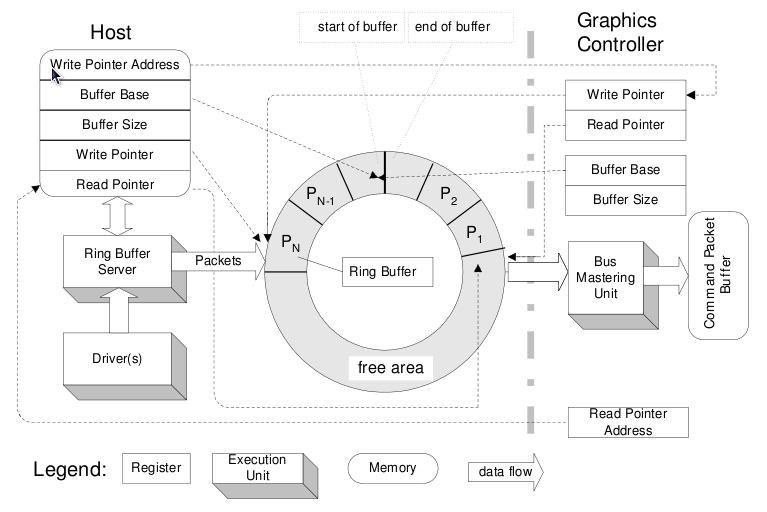
\includegraphics[scale=0.30]{ringbuf.png} \\
		\footnotesize{http://developer.amd.com/gpu\_assets/RRG-216M56-03oOEM.pdf}
	\end{center}
\end{frame}


\begin{frame}[t]{What about the rest of needed functionality?}
	Well, there's no documentation on that.
	\begin{itemize}
		\item A great component of this project is copying logic from the Radeon driver.
		\item Another great component of this project is hope.
	\end{itemize}
\end{frame}



\section{Plan 9 Specifics}

\subsection{Structure of Plan 9 Graphics Drivers}

\begin{frame}[t]{Structure of Plan 9 Graphics Drivers}
	Each Plan 9  graphics driver is split into two components.
	
	\begin{enumerate}
		\pause
		\item kernel component (vgaradeon.c)
		\begin{itemize}
			\item Provides hardware acceleration and blanking.
			\item Drops the card into linear mode.
			\begin{itemize}
				\item The VGA driver handles the actual memory mapping.
			\end{itemize}
		\end{itemize}


		\pause
		\item userspace aux/vga component (radeon.c)
		\begin{itemize}
			\item Reads in BIOS data.
			\item Reads in VGA registers.
			\item Configures and sets VGA registers appropriately.
		\end{itemize}
	\end{enumerate}

	\pause
	Logically, aux/vga executes first.
\end{frame}


\begin{frame}[t]{aux/vga}
	aux/vga represents each video card as a Ctlr. Each Ctlr is an interface providing the following functions:
	\begin{enumerate}
		\pause
		\item options()
		\begin{itemize}
			\item Set values before the init() functions of other Ctlrs are called.
		\end{itemize}

		\pause
		\item init()
		\begin{itemize}
			\item Edit the in-memory copy of the registers to implement the specified mode.
		\end{itemize}
		
		\pause
		\item snarf()
		\begin{itemize}
			\item Read the Ctrl's registers into memory.
		\end{itemize}

		\pause
		\item load()
		\begin{itemize}
			\item Write the Ctrl's modified registers out to the card.
		\end{itemize}
	\end{enumerate}
\end{frame}


\begin{frame}[t]{kernel driver}
	Most interesting logic is handled by the kernel VGA driver.

	The kernel driver for the Radeon is responsible for:
	\begin{itemize}
		\pause
		\item Setting the dedicated mmio regions.
		\pause
		\item Calling the appropriate functions to drop the card and vga driver into linear mode (unless you want segmented mode).
		\pause
		\item Providing hardware acceleration functions.
		\begin{itemize}
			\item In our case, that means using the 3D engine.
		\end{itemize}
	\end{itemize}
\end{frame}


\section{Conclusion}

\subsection{Figures and Estimates}

\begin{frame}[t]{Figures and Estimates}
	The R200/R300 driver is approximately $1,200$ LOC. 
	\begin{itemize}
		\pause
		\item Adding generalized code to enable R200 and R600 in one driver, $+100$.

		\pause
		\item Adding ATOMBIOS to aux/vga: $+10,000$.
		\begin{itemize}
			\item I will attempt to trim it.
			\item The ATI-provided code is actually reasonable.
		\end{itemize}

		\pause
		\item Adding the pull-based ring buffer: $+300$.
		\begin{itemize}
			\item May not be necessary?
		\end{itemize}

		\pause
		\item 3D Engine code: $+2000$ (header files).
	\end{itemize}

	\pause
	Only about $1,500$ lines of actual logic, hopefully.
\end{frame}


\begin{frame}[t]{Order of Operations}
	The project is being completed in roughly the following order:
	\begin{enumerate}
		\pause
		\item Read BIOS data from card (aux/vga).

		\pause
		\item Implement snarf(), then init(), then load().
		\begin{itemize}
			\pause
			\item Test that VGA modesetting works, even if we see garbage.
		\end{itemize}

		\pause
		\item Figure out what kernel bits need to be changed, if any, to get into linear mode.

		\pause
		\item Work on enabling the 3D Engine.
	\end{enumerate}
\end{frame}


\subsection{Questions}

\begin{frame}
	\begin{center}
		questions?
	\end{center}
\end{frame}

\end{document}
